\chapter{Technology: Architecture and Scalability}

\section{Defining a Scalable Tech Strategy}

A scalable technology strategy is foundational to any growing organization. A well-architected strategy ensures that the system can handle increased loads, adapt to changing business requirements, and maintain efficiency as the company evolves. This section explores key elements such as technology selection, evaluation, and future-proofing systems.

\subsection{Technology Selection and Evaluation}

Choosing the right technology stack is critical for long-term scalability and maintainability. The decision-making process should be systematic, taking into account technical and business factors.

\textbf{Key Factors in Technology Selection:}
\begin{itemize}
    \item \textbf{Performance:} Ensuring the selected technology meets required latency and throughput demands.
    \item \textbf{Scalability:} Assessing how well the technology scales horizontally and vertically.
    \item \textbf{Community and Support:} Evaluating the ecosystem, documentation, and vendor support.
    \item \textbf{Security:} Ensuring compliance with industry standards and security best practices \index{security}.
    \item \textbf{Total Cost of Ownership (TCO):} Considering licensing, operational, and maintenance costs.
\end{itemize}

A comparison table can help in technology evaluation:

\begin{table}[ht]
    \centering
    \begin{tabular}{|l|c|c|c|}
        \hline
        \textbf{Criteria} & \textbf{Technology A} & \textbf{Technology B} & \textbf{Technology C} \\
        \hline
        Performance       & High                  & Medium                & Low                   \\
        Scalability       & High                  & High                  & Medium                \\
        Community Support & Strong                & Moderate              & Weak                  \\
        Cost              & Low                   & High                  & Medium                \\
        \hline
    \end{tabular}
    \caption{Technology Selection Matrix}
    \label{tab:tech_selection}
\end{table}

\subsection{Future-Proofing Systems}

Future-proofing technology ensures longevity and adaptability. Some key principles include:

\begin{itemize}
    \item \textbf{Modular Architecture:} Designing systems with clear separation of concerns (e.g., microservices\index{microservices}).
    \item \textbf{Loose Coupling:} Ensuring components communicate via well-defined APIs to minimize dependencies.
    \item \textbf{Backward Compatibility:} Designing systems that support legacy data and integrations.
    \item \textbf{Observability:} Embedding monitoring and logging for proactive issue resolution.
\end{itemize}

\section{Engineering Best Practices}

\subsection{Code Quality and Standards}

Code quality is essential for maintainability and collaboration. Best practices include:

\begin{itemize}
    \item \textbf{Consistent Coding Style:} Using linters and formatters (e.g., Prettier, ESLint).
    \item \textbf{Code Reviews:} Implementing peer reviews to catch bugs early.
    \item \textbf{Documentation:} Maintaining inline and API documentation.
\end{itemize}

\begin{tipbox}
    \textbf{Do not reinvent the wheel:} Programming languages and frameworks have established best practices. Follow them to ensure maintainability and readability.\\
    \\
    \textbf{TypeScript examples:}
    \begin{itemize}
        \item \url{https://docs.aws.amazon.com/prescriptive-guidance/latest/best-practices-cdk-typescript-iac/typescript-best-practices.html}
        \item \url{https://google.github.io/styleguide/tsguide.html}
    \end{itemize}
\end{tipbox}

\subsection{Testing and Automation}

Automated testing improves reliability and efficiency.

\begin{itemize}
    \item \textbf{Unit Tests:} Validating individual components.
    \item \textbf{Integration Tests:} Ensuring components work together.
    \item \textbf{Continuous Integration (CI):} Automating test execution on every commit.
\end{itemize}

\subsection{Security by Design}

Security should be embedded from the start.

\begin{itemize}
    \item \textbf{Threat Modeling:} Identifying potential vulnerabilities.
    \item \textbf{Least Privilege Principle:} Granting only necessary access.
    \item \textbf{Regular Audits:} Conducting security reviews and penetration testing.
\end{itemize}

\section{Infrastructure and Operations}

\subsection{Cloud vs. On-Premise Considerations}

Choosing between cloud\index{cloud} and on-premise\index{on-premise} solutions involves several trade-offs:

\begin{itemize}
    \item \textbf{Scalability:} Cloud solutions offer elastic scaling, whereas on-premise requires capacity planning.
    \item \textbf{Cost:} Cloud follows an OPEX model, while on-premise is typically CAPEX.
    \item \textbf{Control:} On-premise offers greater control over security and compliance.
\end{itemize}

\begin{figure}[h]
    \centering
    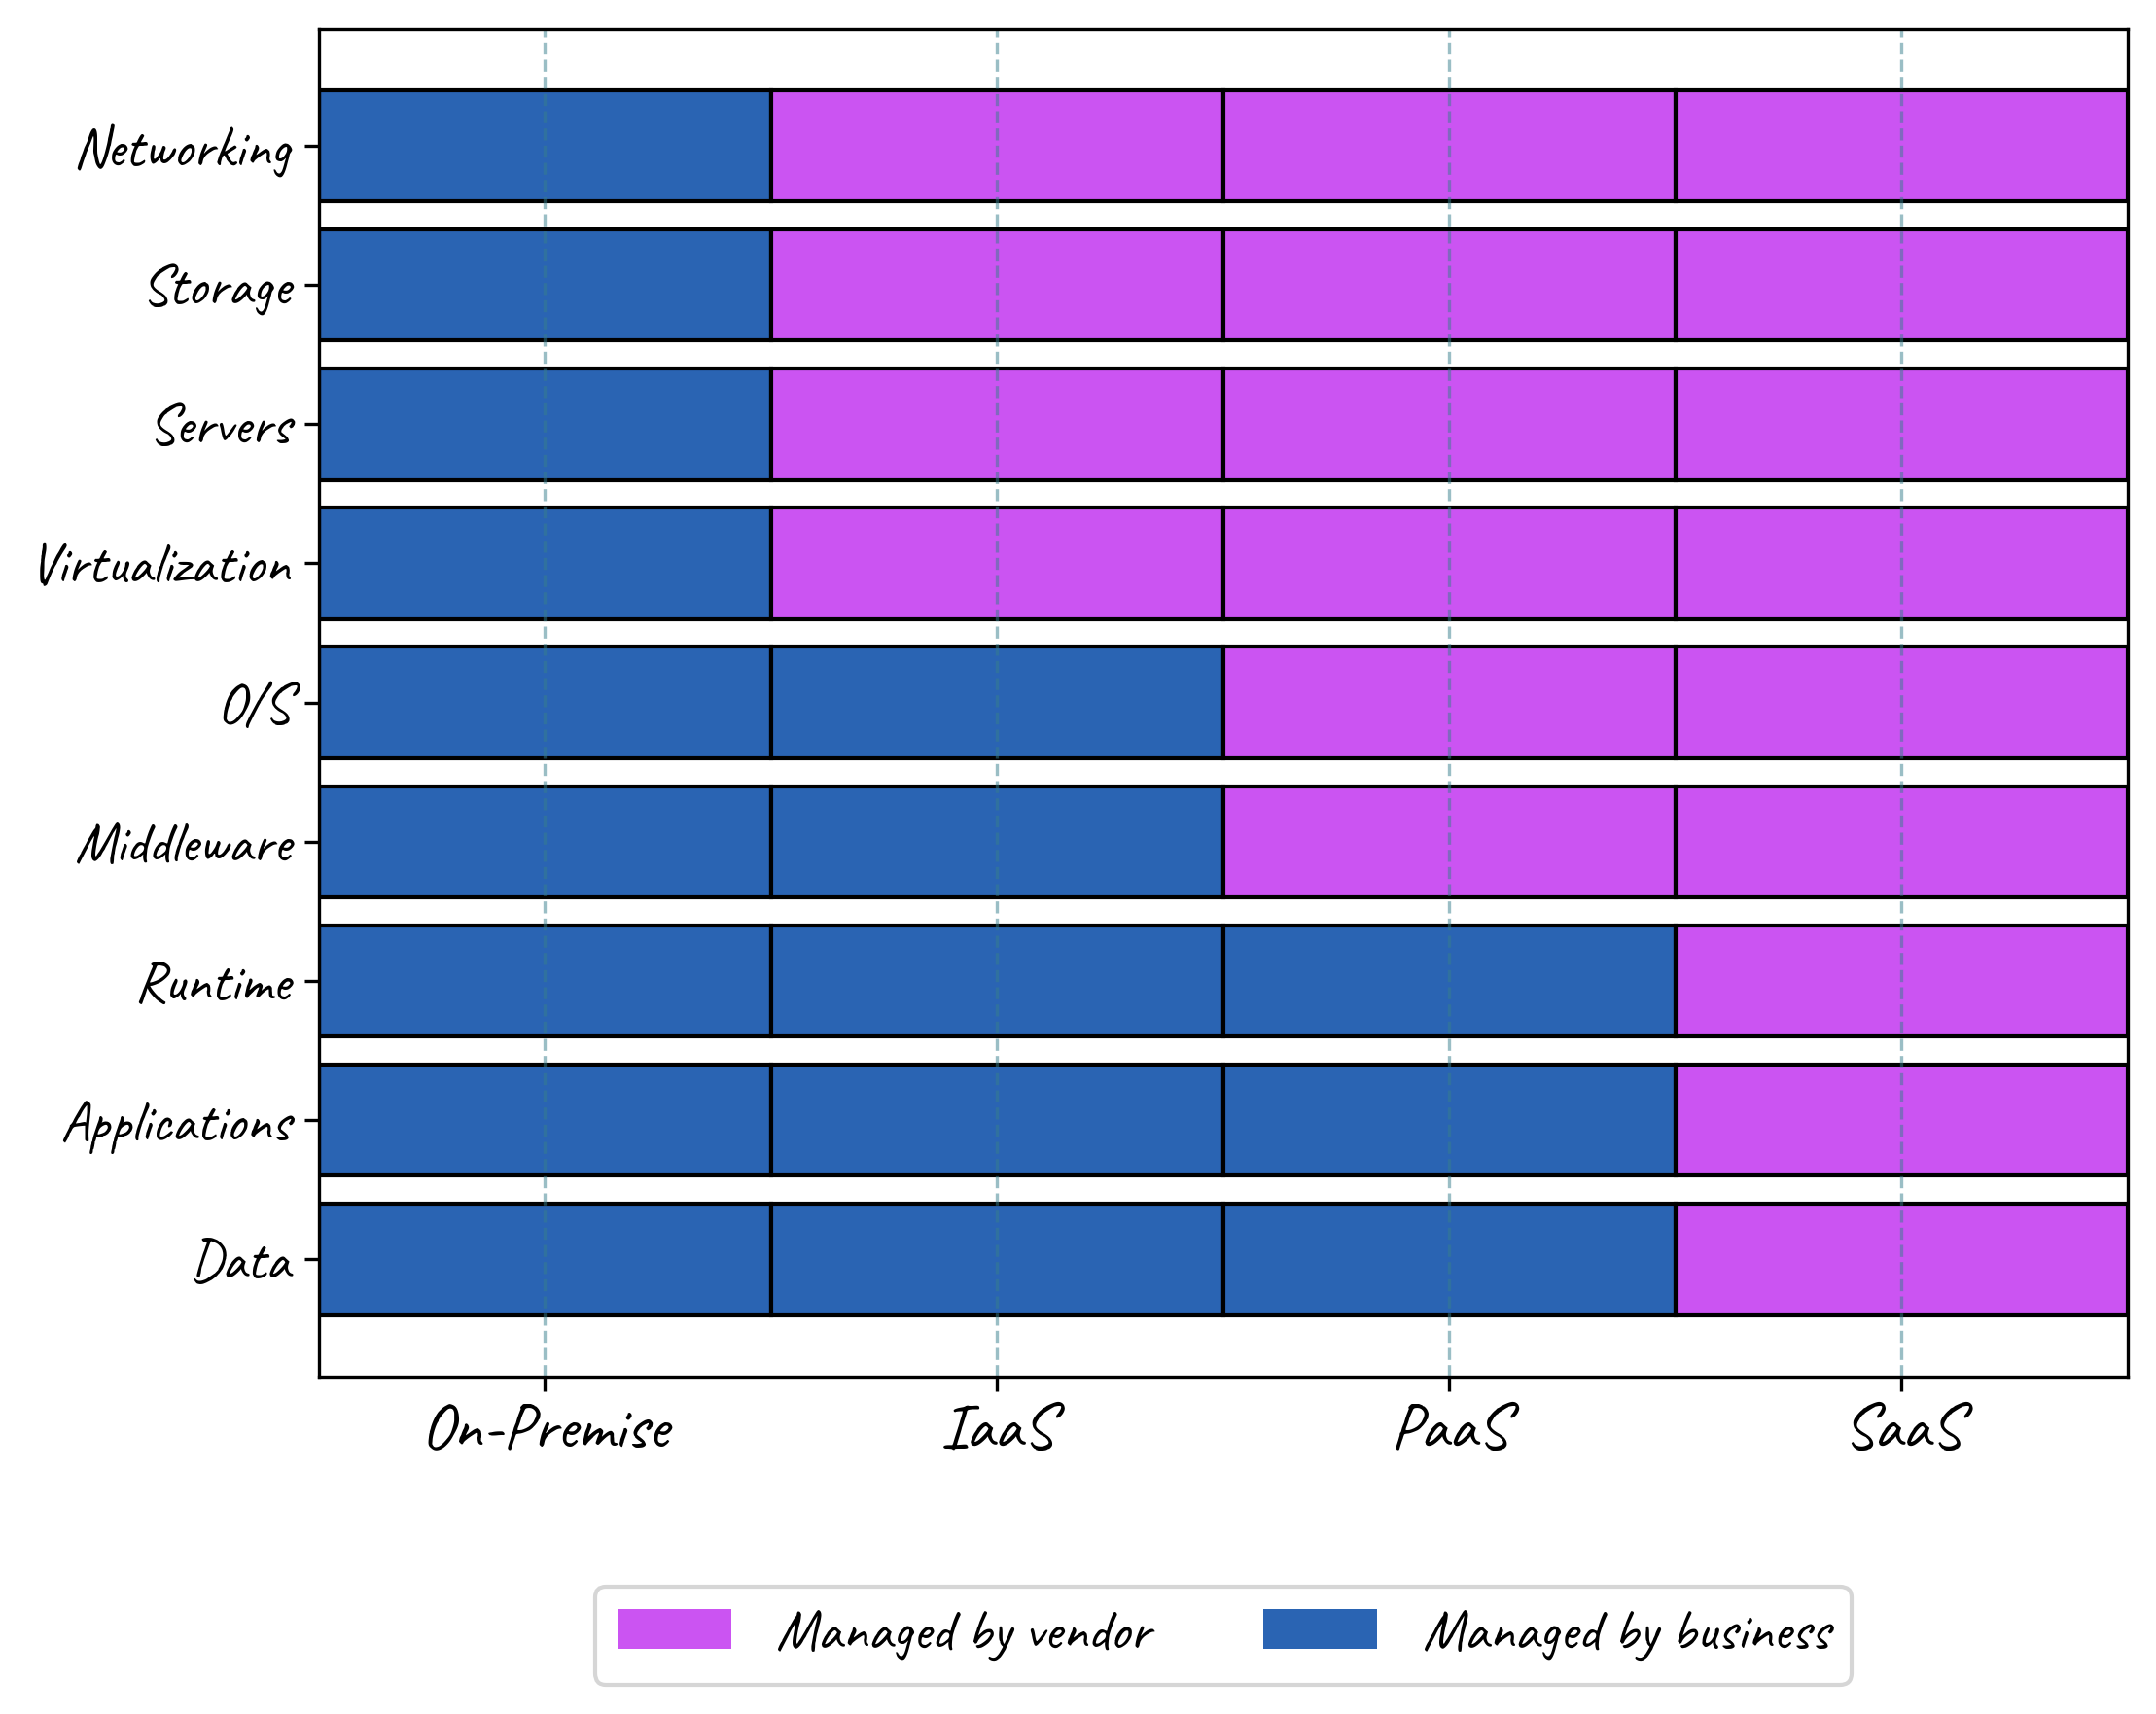
\includegraphics[width=0.8\textwidth]{infrastructure-models.png}
    \caption{Infrastructure models}
\end{figure}

\subsection{Observability and Monitoring}

Monitoring provides visibility into system health. Key components include:

\begin{itemize}
    \item \textbf{Metrics:} Measuring CPU, memory, latency.
    \item \textbf{Logging:} Centralized log aggregation (e.g., ELK stack).
    \item \textbf{Tracing:} Distributed tracing for debugging microservices.
\end{itemize}

\subsection{Incident Management and Reliability}

A structured approach to incident response improves reliability.

\begin{itemize}
    \item \textbf{Incident Response Plan:} Predefined escalation paths.
    \item \textbf{Postmortems:} Learning from past failures.
    \item \textbf{Redundancy:} Designing failover and high-availability systems.
\end{itemize}

This structured approach ensures scalable, resilient technology that supports long-term business growth.
